%%%%%%%%%%%%%%%%%%%%%%%%%%%%%%
%
%\BiChapter{基于聚焦感知的光场显著性目标检测}
%{Light Field Salient Object Detection Based on Focus Perception}
%
%\BiSection{研究动机}{Research Motivation}
%
%
%\BiSection{方法介绍}{Method Introduction}
%\BiSubsection{令牌通信模块}{Token Interaction Module}
%\BiSubsection{聚焦感知增强策略}{Focus Perception Enhancement Strategy}
%\BiSubsection{训练过程}{Training Process}
%
%
%\BiSection{实验结果与分析}{Experimental Results and Analysis}
%\BiSubsection{实验设置}{Experimental Setup}
%\BiSubsection{消融实验}{Ablation Experiment}
%\BiSubsection{对比实验}{Comparative Experiment}
%
%
%%%%%%%%%%%%%%%%%%%%%%%%%%%%%%%%%%%%%%%%%%%%%%%%%%%%%%%%%%%%%%%%%%%%%%%%%%%%%%




%%%%%%%%%%%%%%%%%%%%%%%%%%%%%%%%%%%%%%%%%%%%%%%%%%%%%%%%%%%%%%%%%%%%%%%%%%%%%%
\BiChapter{基于聚焦感知的光场显著性目标检测}
{Light Field Salient Object Detection Based on Focus Perception}
\label{chap:part3}
%
%
光场显着物体检测(LFSOD)由于光场中包含丰富的空间信息而引起了广泛的关注。
与 2D (RGB) 和 3D (RGBD) 数据不同,光场本质上捕获结构化 4D 表示,包括多视图图像、深度图和焦点切片。 其中,通过眼球运动顺序观察切片的焦点堆栈,
以及迎合人类视觉感知的可见注意力转移\upcite{piao2020dut},做出适合显着性对象检测。





%%%%%%%%%%%%%%%%%%%%%%%%%%%%%%%%%%%%%%%%%%%%%%%%%%%%%%%%%%%%%%%%%%%%%%%%%%%%%%
\BiSection{研究动机}{Research Motivation}


一些开创性的方法\upcite{zhang2019memory,piao2020exploit}采用 ConvLSTM\upcite{shi2015convolutional},
它使用记忆机制以预定义的顺序单独处理焦点堆栈特征。
张等人\upcite{zhang2021learning}后来在编码器阶段采用3D卷积来提取特征。
刘等人\upcite{liu2021light}和
张等人\upcite{zhang2021geometry}使用图神经网络来聚合不同焦点切片中的上下文信息。 
这些方法依赖内存使用或大量计算来提取焦点堆栈特征,从而限制了效率。




%---------------------------------------------------------------------> fig: 创新图
\begin{figure}[!ht]
	\centering
	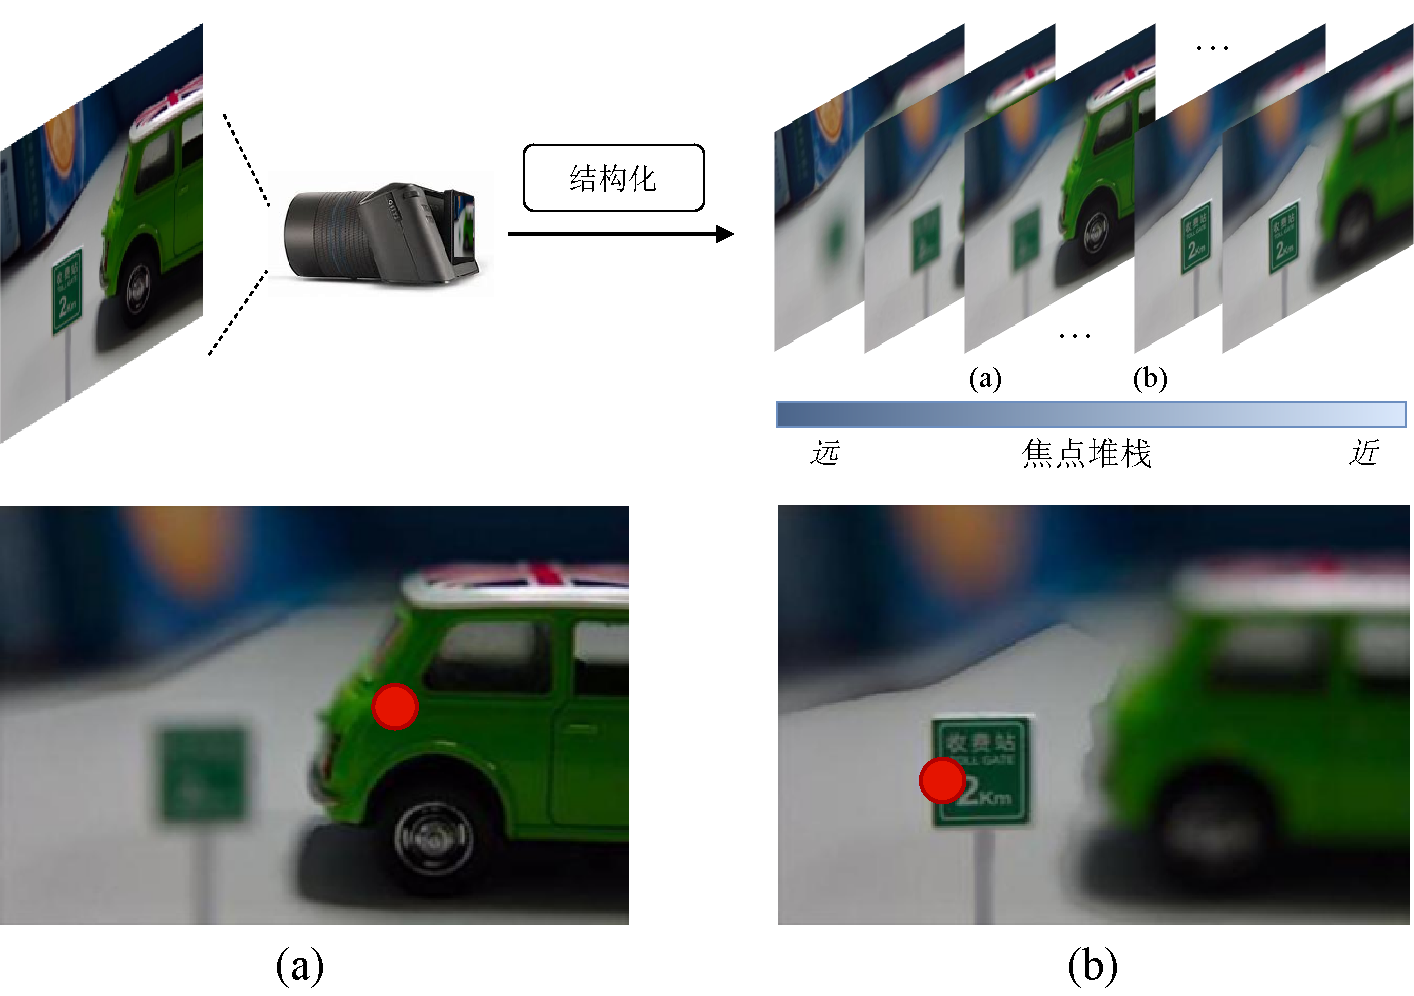
\includegraphics[width=0.85\linewidth]{figures/chapter3/cpt3_idea.pdf}
	\bicaption{光场焦点堆栈的成像过程和不同切片的成像效果}
	{The imaging process of the light field focus stack and the imaging effects of different slices}
	\label{figure:cpt3:idea}
\end{figure}




本章重新思考光场数据建模的方式。考虑到焦点堆栈的成像效果,如图~\ref{figure:cpt3:idea}~所示,每个焦点切片根据空间透视深度的不同,聚焦部位也不同。 并且从同一场景生成,焦点切片有很多共同点。
因此,即使在很小的带宽内,也可以充分总结和传达它们之间的差异。 此外,给定图像,人类可以毫不费力地关注敏感部分并忽略不重要的背景。 因此,在焦点堆栈中处理更多相对的焦点切片来模拟人类视觉系统是合理的。 


受上述观察的启发,考虑两个关键问题:
1)如何设计一个模型来存储切片级特征并在焦点堆栈和全焦点图像之间传递信息以进行上下文建模? 
2)如何设计一个模型来理解场景的空间分布并感知敏感的焦点切片? 

在本章中,提出了一种用于高效且有效的 LFSOD 的聚焦感知Transformer(FPT)。 
具体来说,通过收集图像特定的特征并制定通信以加强焦点堆栈和全焦点图像之间的相互感知。 
通过利用选择性机制将适当的焦点切片纳入检测。 
具体来说,本章的贡献有三个:



\begin{itemize}
	\item 引入与焦点相关的标记来总结图像特定的特征,并提出一种标记通信模块(TCM),通过计算与焦点相关的标记之间的交叉注意力来执行特征交互。 通过转移焦点堆栈中与焦点相关的标记来促进空间上下文传播。 
	
	\item 提出了一种聚焦感知增强(FPE)策略,通过切片选择机制来增强焦点堆栈中的特征空间表示,以有区别地处理适当的焦点切片。	这可以突出显着切片并抑制非显着区域的干扰。 
	
	\item 在 4 个广泛使用的数据集进行了广泛的实验,
	并证明本章所提方法优于现有最先进的光场显著性目标检测方法。 本章所提出的方法在 DUTLF-FS\upcite{zhang2019memory}上将 MAE 指标显着降低了 31\%。
\end{itemize}







%%%%%%%%%%%%%%%%%%%%%%%%%%%%%%%%%%%%%%%%%%%%%%%%%%%%%%%%%%%%%%%%%%%%%%%%%%%%%%
\BiSection{方法介绍}{Method Introduction}


\begin{figure}[!ht]
	\centering
	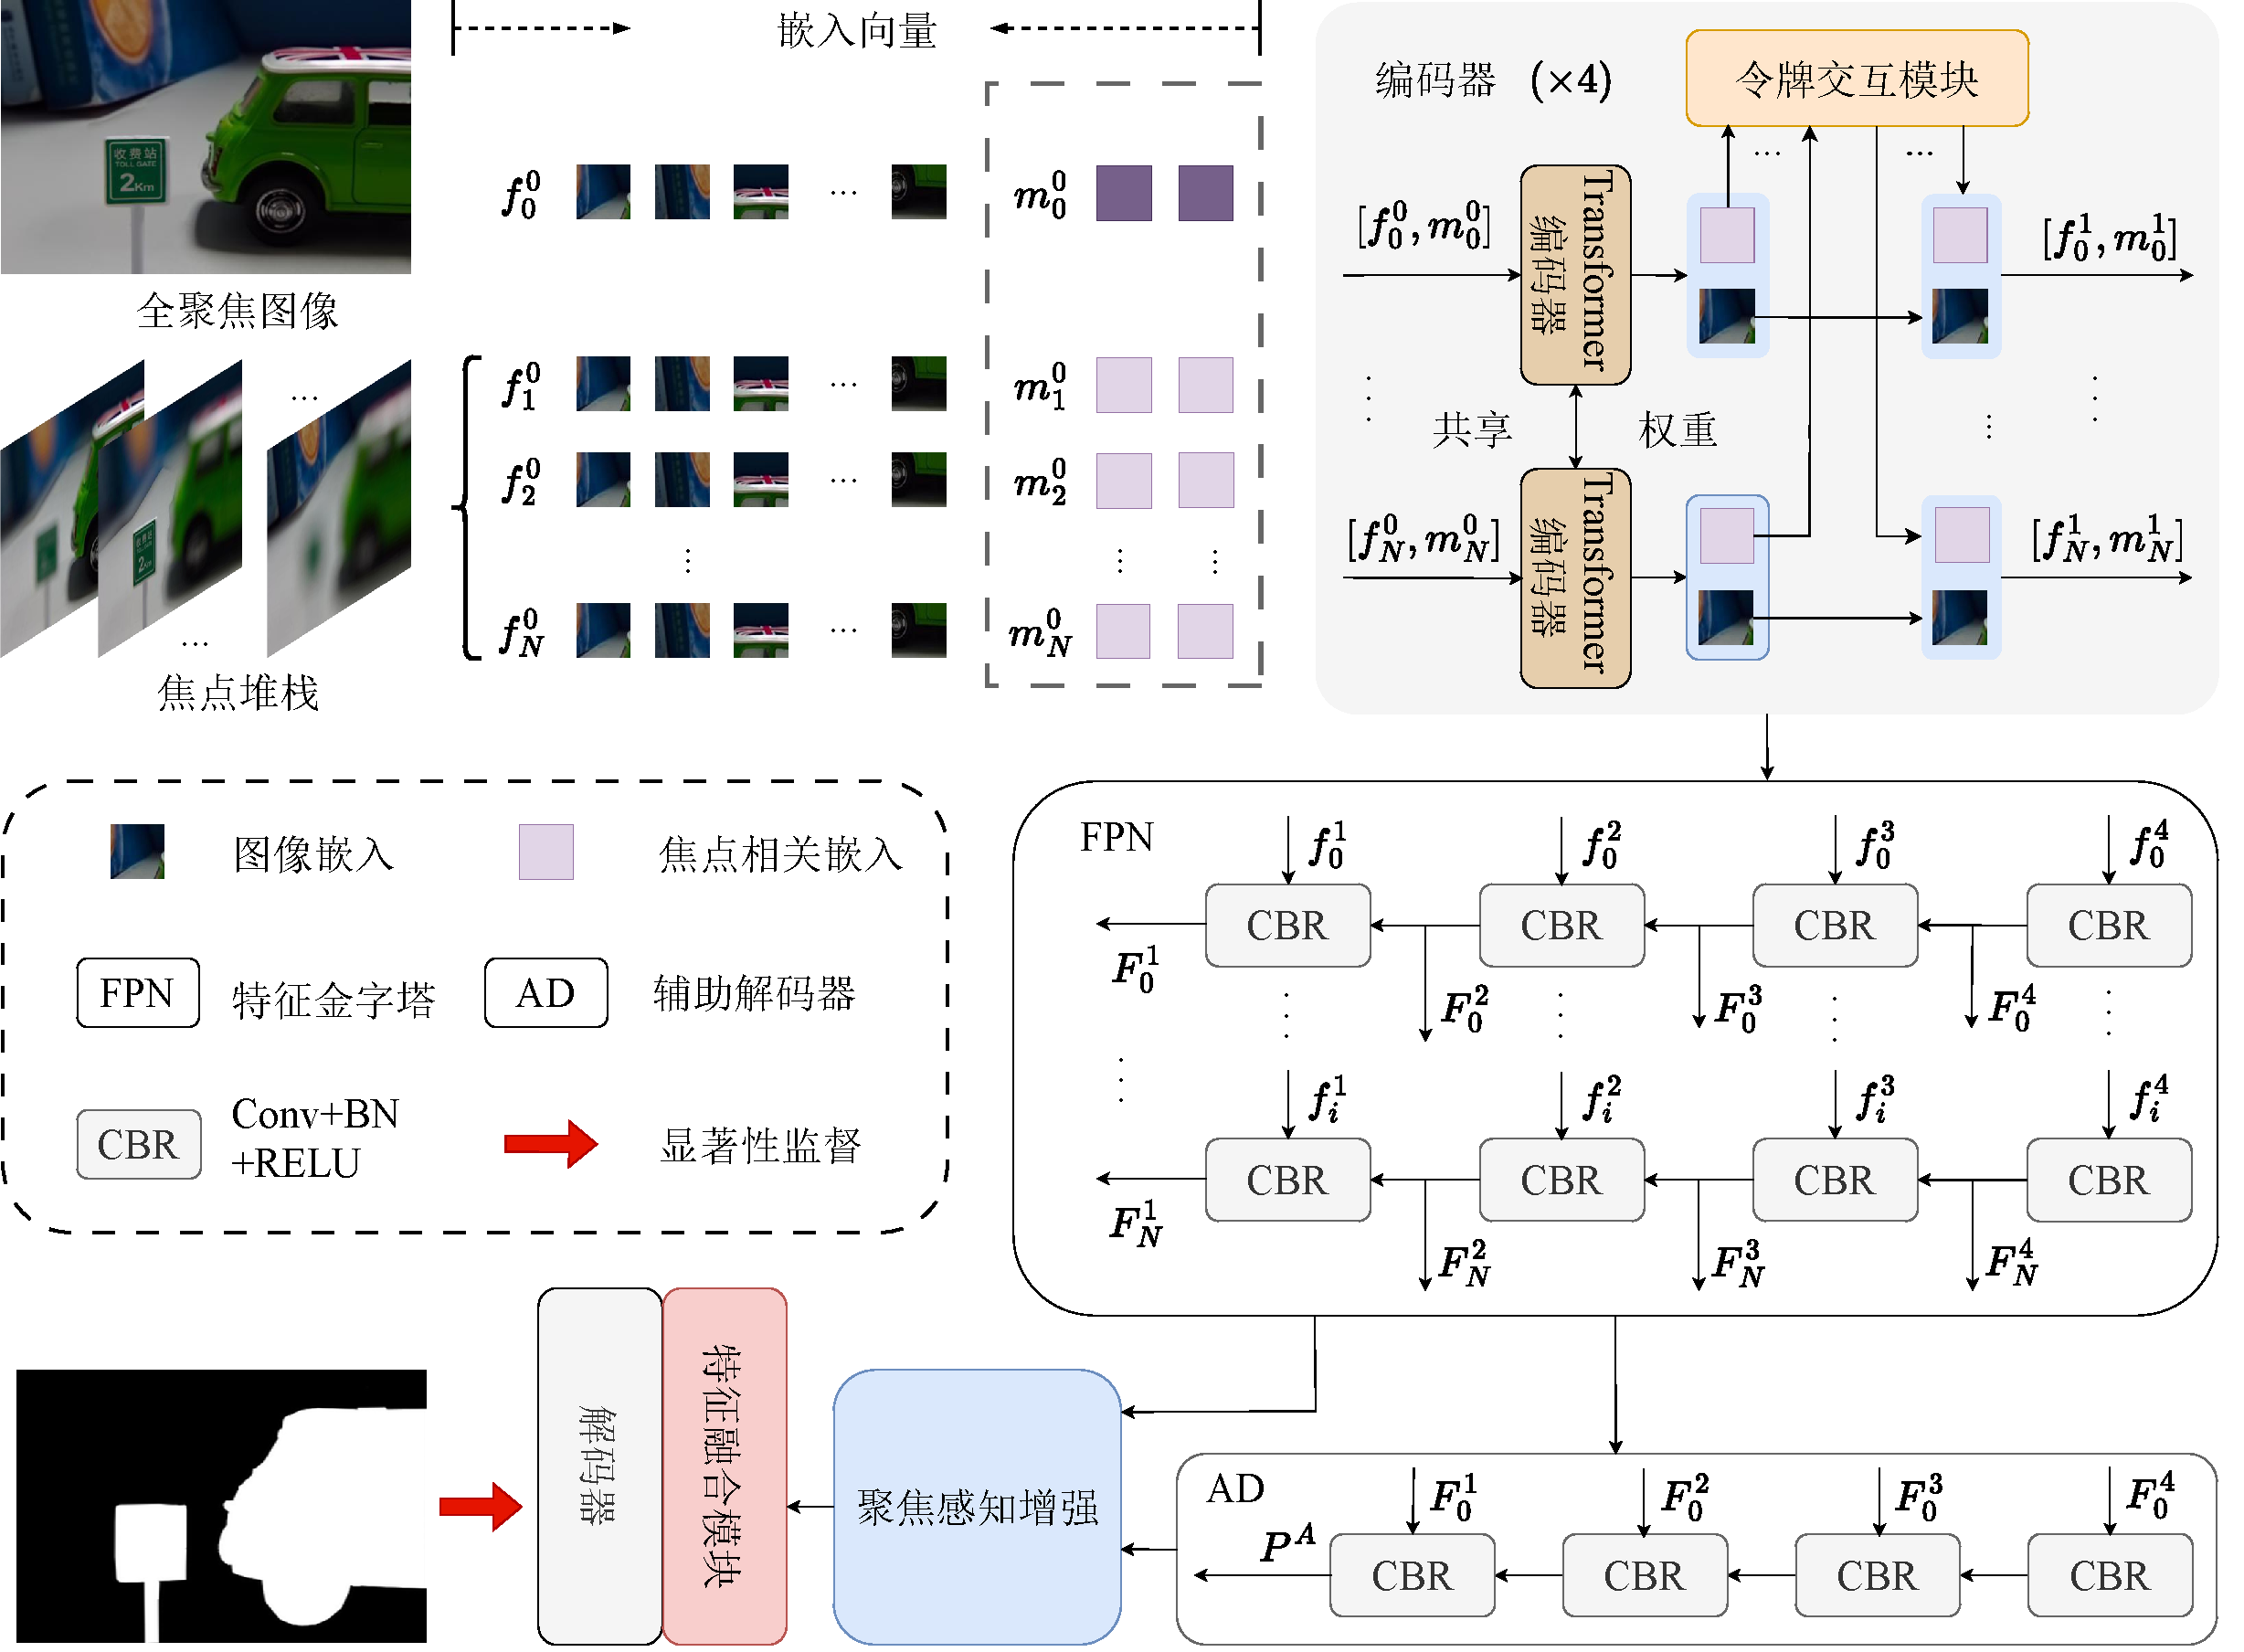
\includegraphics[width=0.95\linewidth]{figures/chapter3/overview_1}
	\bicaption{光场显著性目标检测网络结构图}
	{The architecture of light field salient object detection network}  
	\label{cpt3_fig1:overview}
\end{figure}




本章方法所提出的聚焦感知Transformer的整体架构如图~\ref{cpt3_fig1:overview}~所示。
给定 $N + 1$ 个分辨率为 $ H \times W $ 的图像,包括一个全焦点图像和 $N$ 个焦点堆栈图像,将每个图像划分为补丁区块作为输入。 
将展平的 $N$ 个 patch 输入到线性投影中,得到嵌入的 patch $ \left \{ f_{i}^{0} \right \}_{i=0}^{N} $,其形状为$ \left ( N + 1 \right ) \times \frac{HW}{P^{2}} \times C  $,其中 $P$ 表示每个 patch 的大小,$C$ 表示每个 patch 的大小。 
渠道维度。 
%
%
%
具体地,$ f_{0}^{0} $ 表示全焦点图像的特征输入。 
$ \left \{ f_{i}^{0} \right \}_{i=1}^{N} $ 表示焦点堆栈的特征输入。 
此外,为了总结补丁中的信息,引入了一组大小为 $ M \times C $ 的随机初始化的可学习嵌入,作为 { }N 个焦点相关标记,表示为 $ \left \{ m_{i}^{0} \right \}_{i=0}^{N} $ ,其中 $M$ 表示焦点相关标记的数量。 
将每个 patch 的与焦点相关的标记连接起来,
并得到 $ \left \{ \left [ f_{i}^{0},m_{i}^{0}  \right ]  \right \}_{i=0}^{N} $ 作为特征提取器的输入。 




与卷积网络使用不同的卷积步长来获得多尺度特征图不同,
本章方法使用渐进收缩策略,通过patch嵌入层来控制特征图的尺度。
用$ l \in 1..T $ 表示阶段编号。 
将第$l$个阶段补丁块大小表示为$P_{l}$,在第$l$阶段开始时,
首先均匀划分输入特征图
$F_{l-1} \in \mathbb{R}^{H_{l-1} \times W_{l-1} \times C_{l-1}}$
为
$ \frac{H_{l-1}W_{l-1}}{P_{l}^{2}} $
个补丁块。




然后,将每个补丁块展平并投影到$C_{l}$维度的嵌入表达。
在线性投影之后,嵌入补丁的形状可以看做是
$\frac{H_{l-1}}{P_{l}} \times \frac{W_{l-1}}{P_{l}} \times C_{l} $,
其中高度和宽度比输入小了$P_{l}$倍。
这样就可以灵活调整每个阶段的特征图的尺度,
使得可以构建基于Transformer的特征金字塔。
%
%
%
%
第$l$阶段的Transformer编码器有 $ N_{i} \in [3,4,6,3] $ 个 Transformer 块。
%
%
%
%
%
%\par
\begin{figure}[!ht]
	\centering
	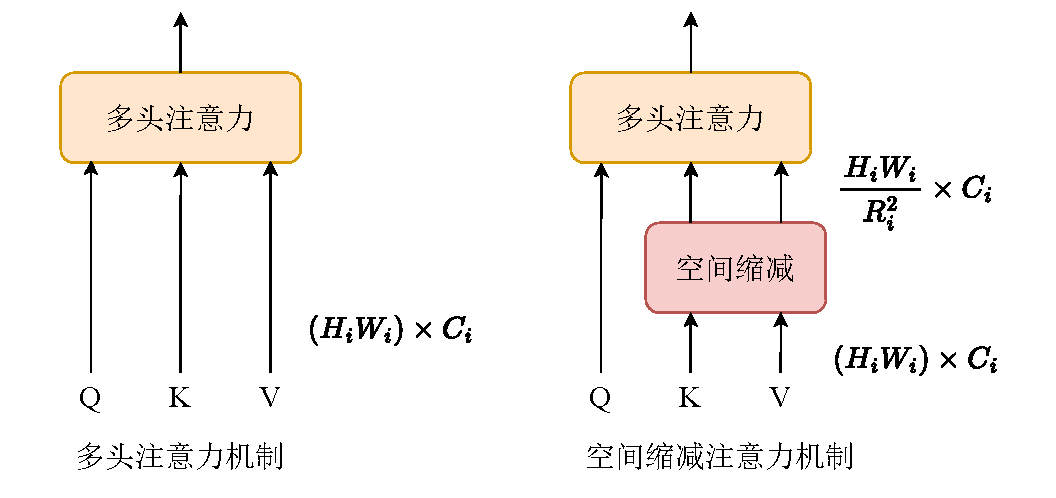
\includegraphics[width=0.95\linewidth]{figures/chapter3/sra}
	\bicaption{多头注意力与空间缩减注意力}
	{Multi-head attention (MHA) vs spatial reduction attention (SRA)}  
	\label{cpt3_fig1:sra}
\end{figure}




本章方法构造了基于金字塔Transformer(Pyramid Vision Transformer,PVT)
\upcite{wang2022pvt}的主干网,共由 $T = 4$ 个阶段组成。 
骨干网络需要从原始高尺寸输入开始处理,一步步获取不同尺度的特征表示。
本章方法采用空间缩减注意力(Spatial-Reduction Attention,SRA)来取代Transformer编码器\upcite{vaswani2017attention}中传统多头注意力(Multi-Head Attention)层。



与多头注意力机制类似,空间缩减注意力接受查询$Q$、秘钥$K$和值$V$作为输入,并细化输出的特征。
不同之处在于,仅需注意力操作之前缩减了$K$和$V$的空间尺度,如图~\ref{cpt3_fig1:sra},
能够在很大程度上减少计算和内存开销。
第$l$阶段的空间缩减注意的具体实现过程如下:
%
%
%
%
\begin{equation}
	SRA(Q,~K,~V) = Concat(head_{0},~ \cdots,~ head_{H_{l}})~W^{O}
\end{equation}
%
%
\begin{equation}
	head_{j} = Attention(Q~W_{j}^{Q}, ~ SR(K)~W_{j}^{K},~ SR(V)~W_{j}^{V})
\end{equation}
%
%
%
其中$Concat(\cdot)$是连接操作。
$W_{j}^{Q} \in \mathbb{R}^{C_{i} \times d_{head}},~
W_{j}^{K} \in \mathbb{R}^{C_{i} \times d_{head}},~
W_{j}^{V} \in \mathbb{R}^{C_{i} \times d_{head}},~$
和
$W^{O} \in \mathbb{R}^{C_{i} \times C_{i}}~$
是线性映射参数。
$H_{l}$是每个阶段注意力层的头数。
$SR(\cdot)$是减少输入序列空间维度的操作,它的公式是:
%
%
%\\
%
\begin{equation}
	SR(x) = Norm(Reshape(x, R_{l})W^{S})
\end{equation}
%
%
其中$x \in \mathbb{R}^{(H_{l}W_{l}) \times C_{l}} $
表示输入序列,$R_{l}$表示每个阶段中的注意力层的缩减比例。
$Reshape(x, R_{l})$ 表示将输入序列 $x$ 重塑大小为
$\frac{H_{l}W_{l}}{R_{i}^{2}} \times (R_{i}^{2}C_{i})$。
$W_{S} \in \mathbb{R}^{R_{i}^{2}C_{i}}$
是一个线性投影,它将输入序列的维度减少到$C_{l}$。
$Norm(\cdot)$指的是层归一化。
%
%
\par
%
%
与原始的Transformer\upcite{vaswani2017attention}中一样,
本章所提网络中每个 Transformer 块包括线性空间减少注意力 (SRA) 和前馈网络 (FFN),
以每个图像的方式作用于联合注意学习:
%%
%%
\begin{equation}
	\left \{ [f_{i}^{l}, m_{i}^{l}]\right \}_{i=0}^{N} = \left \{ FFN^{l} \left  ( SRA^{l} \left ( [f_{i}^{l-1}, m_{i}^{l-1}]\right )\right )\right \}_{i=0}^{N},
\end{equation}
%%
%%
每个Transformer编码器后面都布置了令牌通信模块(TCM),用于特征通信。 













经过特征提取,从 Transformer 块的输出中得到四层特征 
$\left \{ f_{i}^{1},f_{i}^{2},f_{i}^{3},f_{i}^{4} \right \}_{i=0}^{N}$ 。 
之后,采用共享权重特征金字塔网络(FPN)\upcite{lin2017feature}进行分层融合并得到 $N$ 个金字塔特征图	$ \left \{F_{i}^{1},F_{i}^{2},F_{i}^{3},F_{i}^{4} \right \}_{i=0}^{N}$:
%%
%%
\begin{equation}
	\begin{aligned}
		F_{i}^{4} &= Up \left ( CBR \left ( f_{i}^{4} \right )\right ) \\ 
		F_{i}^{l} &= Up \left ( CBR \left ( f_{i}^{l} + F_{i}^{l+1} \right )  \right ),l=1,2,3  .
	\end{aligned}
\end{equation}
%%
%%
其中 $Up$ 贡献 $2 \times $ 上采样 操作时,$CBR$ 表示一个卷积块,包括 Conv+ BN+ RELU 层。 对于解码器,提出的聚焦感知增强(FPE)策略增强了焦点堆栈的特征表示。 增强的焦点堆栈和全焦点特征融合在特征融合模块(FFM)中。 最后,采用掩模解码器来生成显着图。

















%%%%%%%%%%%%%%%%%%%%%%%%%%%%%%%%%%%%%%%%%%%%%%%%%%%%%%%%%%%%%%%%%%%%%%%%%%%%%%
\BiSubsection{令牌通信模块}{Token Interaction Module}



\begin{figure}[b]
	\centering
	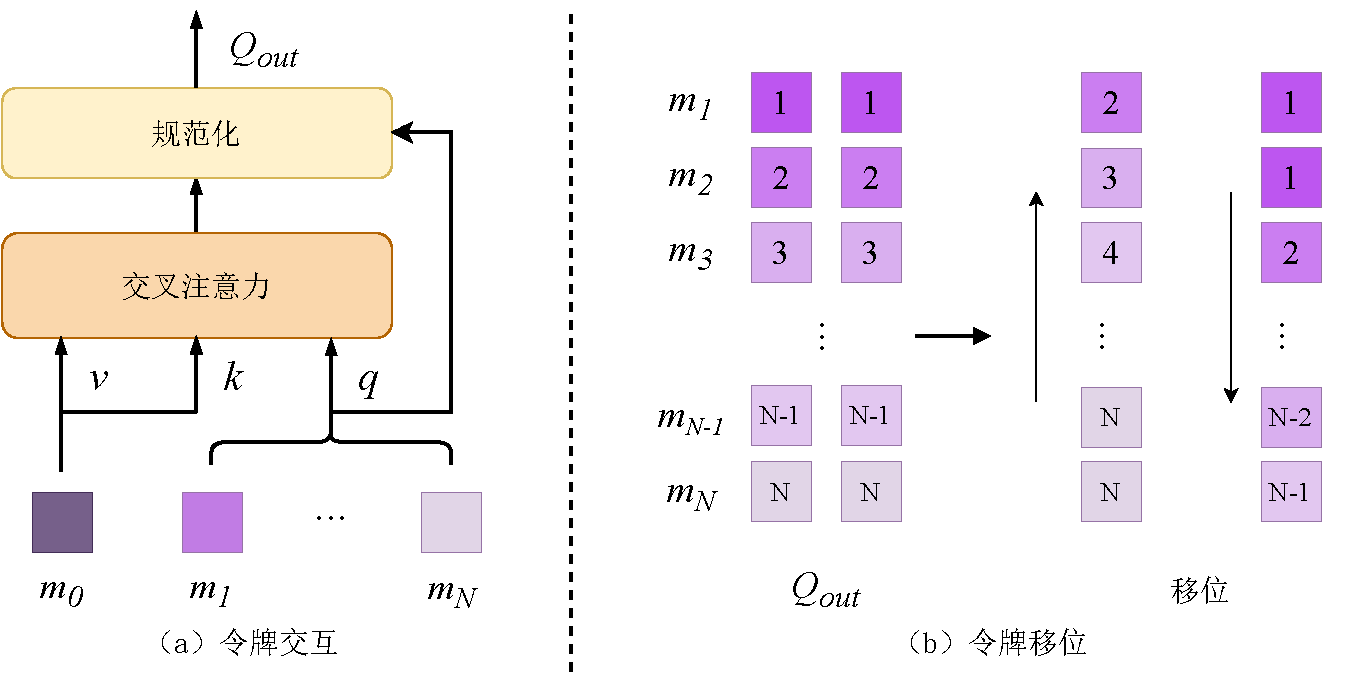
\includegraphics[width=0.95\linewidth]{figures/chapter3/token-interaction.drawio}
	\bicaption{令牌通信模块的框架流程图}
	{Framework diagram of the token communication module}
%	{令牌通信模块}
%	{An illustration of the Token Communication Module (TCM)}  
	\label{cpt3_fig1:token_interaction}
\end{figure}



在以前的光场显著性检测方法中,主干网络仅以原像方式执行特征提取\upcite{piao2020exploit, liu2021light},忽略了光场数据固有的丰富上下文信息。 相比之下,本章方法设计了一个令牌通信模块(Token Communication Module,TCM)来对全焦点和焦点堆栈进行上下文建模,如图~\ref{cpt3_fig1:token_interaction}~所示。
TCM 由令牌交互(Token Interaction,TI)和令牌移位(Token Shift,TS)操作组成。 
令牌通信模块在全焦点和焦点堆栈的焦点相关令牌之间进行交叉注意力计算,以进行信息交互。 
令牌移位操作通过转移焦点堆栈中与焦点相关的标记,以促进上下文特征感知。 








%%%%%%%%%%%%%%%%%%%%%%%%%%%%%%%%%%%%%%%%%%%%%%%%%%%%%%%%%%%%%%%%%%%%%%%%%%%%%%%%%%%%
(1)
令牌交互操作


如图~\ref{cpt3_fig1:token_interaction}~(a)~所示,令牌交互由交叉注意力 (Cross Attention,CA) 块组成。 
注意力函数可以描述为将查询和一组键值对映射到计算为值的加权和的输出。 
分配给每个值的权重是查询与相应键之间的相似度。 
这里,采用带有残差连接和层归一化的缩放点积注意力来实现交叉注意力块,公式可以表述如下:
%\todo
%
%
%
%%
\begin{equation}
	Attention(Q,K,V) = softmax \left ( \frac{QK^{T}}{\sqrt{d_{k}}} \right ) V,
\end{equation}
%%
%%
%
%
其中
$ Q \in \mathbb{R}^{N_{q}\times d_{k}}  $,
$ K \in \mathbb{R}^{N_{k}\times d_{k}}  $ 和
$ V \in \mathbb{R}^{N_{v}\times d_{k}}  $ 
分别是查询、键和值。 
$ d_{k} $ 是查询和密钥的通道维度,
$ \sqrt{d_{k}} $ 是控制softmax分布的温度参数。 
对于交叉注意力块,$K$ 和 $V$ 是相同的。 






交叉注意力块将所有与焦点相关的标记 $ \left \{ m_{i}^{l} \right \}_{i=0}^{N} $ 作为输入。 焦点堆栈流的标记 $ \left \{  m_{i}^{l} \right \}_{i=1}^{N} $ 用作查询来计算与属于全焦点流的键 $ m_{0}^{l} $ 的相似度并从值 $ m_{0}^{l} $ 检索焦点信息。 该交叉注意力块的输出 $ Q_{out}^{l} $ 可计算如下:
%
%
%%
%%
\begin{equation}
	Q_{out}^{1} = LN \left ( Attention(Q,K,V) + Q \right ),
\end{equation}
%%
%%
%
%
其中
$ Q = \left \{ m_{i}^{1} \right \}_{i=1}^{N}~ W^{Q}$,
$ K= m_{0}^{1} ~W^{K} $,
$ V =  m_{0}^{1}~ W^{V} $。
$ Q$,$K$,$V$ 和 $ Q_{out}^{l} $
的维度分别为 
$ N \times M \times C $,$ M \times C $,$ M \times C $ 
和
 $ N \times M \times C $。 


















%%%%%%%%%%%%%%%%%%%%%%%%%%%%%%%%%%%%%%%%%%%%%%%%%%%%%%%%%%%%%%%%%%%%%%%%%%%%%%%%%%%%
(2)
令牌移位操作




上述操作的输出 $ Q_{out}^{l} $ 被馈送到令牌移位操作中,
如图~\ref{cpt3_fig1:token_interaction}~(b)~中所示。 
与焦点相关的标记被分为 $G = 2$ 组,并沿着焦点深度轴以不同方向(向前或向后)移动。 
对于每组焦点相关嵌入表示,可以看做是整体往左(或右)移动了一个图像级切片的位置。
经过一次移位操作,
每一张切片所对应的焦点相关嵌入由其左右两张切片的焦点相关嵌入的共同组合,
而对于两端的散焦切片,只汇总了一个方向上的不同图片的焦点相关嵌入信息。




通过不同的焦点深度和方向,令牌可以实现与近深度和远深度焦点图像的空间特征进行上下文交换。 
然后用连接的 $ \left \{ m_{i}^{l} \right \}_{i=0}^{N} $ 更新所有与焦点相关的标记  $ \left \{ m_{i}^{l} \right \}_{i=0}^{N} $ 并将 
$ Q_{out}^{l} $ 移出。 
%
%
%\\
%
%
%\par
%
%
这种设计的目的是随着网络的深入,能够促进网络对于光场三维场景的整体感知,
从而保持稳定的空间感受野。 
值得一提的是,令牌移位操作几乎是无参数的,带来的计算成本可以忽略不计。







%%%%%%%%%%%%%%%%%%%%%%%%%%%%%%%%%%%%%%%%%%%%%%%%%%%%%%%%%%%%%%%%%%%%%%%%%%%%%%%%%%%%%%%%%%
\BiSubsection{聚焦感知增强策略}{Focus Perception Enhancement Strategy}



受人类视觉注意系统中关注选择性的启发,本章方法的目标是从多焦点特征中有效地感知有用的显着性信息。 
本章提出了一种聚焦感知增强(Focus Perception Enhancement,FPE)策略来模仿人类如何从视觉资源中选择感兴趣信息的筛选阶段。 
聚焦感知增强策略由切片选择机制组成,
用于有区别地处理焦点相关切片,
如图~\ref{cpt3_fig1:fpe}~所示。
选择机制可以突出显着切片并抑制非显着区域的干扰。 
此外,本章采用结构相似性\upcite{wang2003multiscale}来评估焦点切片和全焦点图像之间焦点的一致性,
因为散焦状态下的物体不具有清晰的纹理结构。 



\begin{figure}[!ht]
	\centering
	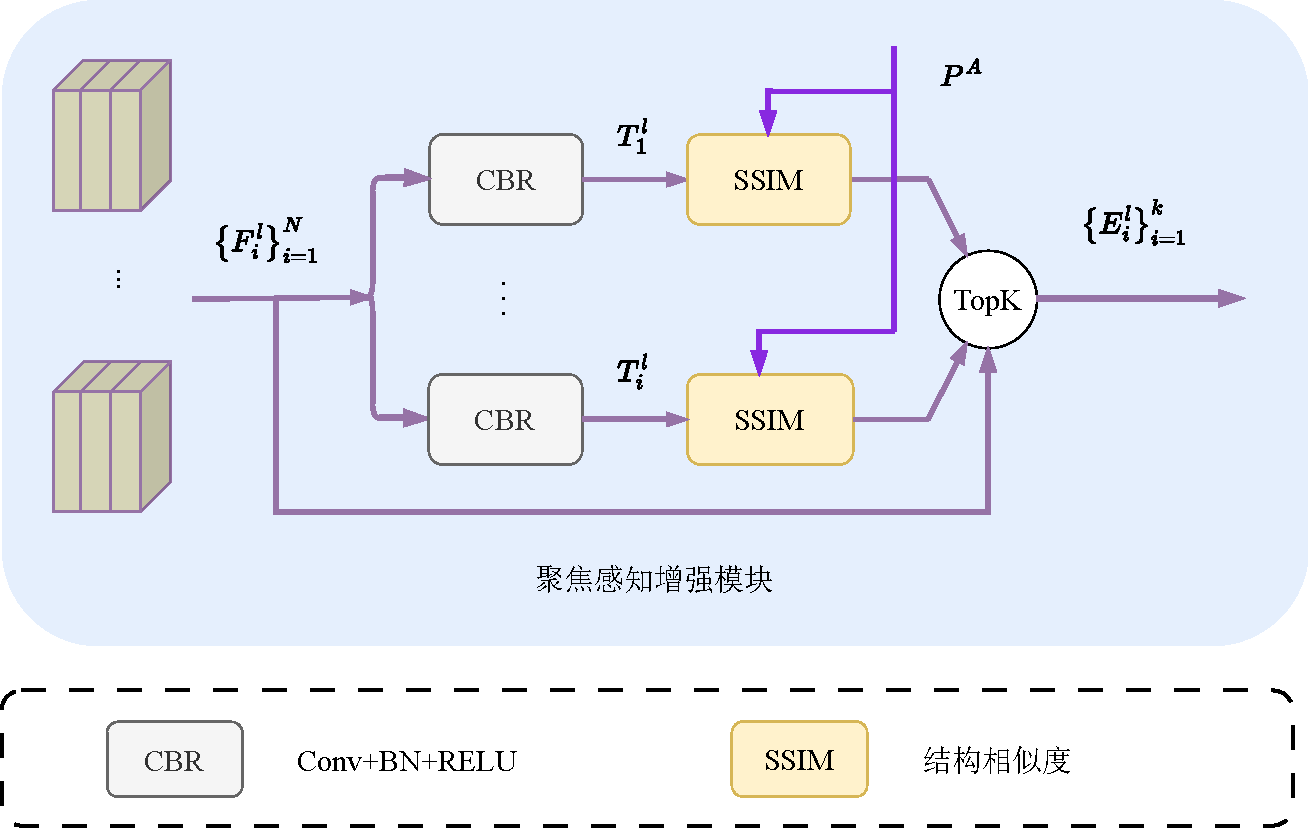
\includegraphics[width=0.90\linewidth]{figures/chapter3/fpe}
	\bicaption{聚焦感知增强策略的流程图}
	{Structural diagram of the focus perception enhancement module}
	\label{cpt3_fig1:fpe}
\end{figure}



首先,使用基于特征金字塔网络的辅助解码器(Auxiliary Decoder,AD)
生成辅助显着性预测 $ P^{A} $ 并应用监督以避免非显着对象的干扰并确保全焦点特征的有效性。 
然后,使用全焦点显着性预测 $ P^{A} $ 计算焦点堆栈 $ \left \{ F_{i}^{l} \right \}_{i=1}^{N} $ 的每个层特征的结构相似度得分。 
%%
%%
\begin{equation}
	score_{i}^{l} = SSIM \left ( CBR \left ( F_{i}^{l} \right ), P^{A} \right ),
\end{equation}
%%
%%
%
%
其中 $CBR$ 表示一个卷积块,它将特征通道压缩成一维。 $SSIM$ 表示结构相似度,可以表示为: 
%
%
%%
%%
\begin{equation} 	
	SSIM(x,y)=\frac{\left ( 2\mu_{x}\mu_{y}+C_{1} \right ) \left (  2\sigma_{xy}+C_{2} \right )  } 	
	{\left ( \mu_{x}^{2} + \mu_{y}^{2}+C_{1}\right ) \left ( \sigma_{x}^{2}+ \sigma_{y}^{2} + C_{2} \right ) } , 	
\end{equation}
%%
%%
其中 $x$ 和 $y$ 表示两个输入图像,$\mu_{x}$、$\mu_{y}$ 和 $\sigma_{x}$ , $\sigma_{y}$分别是$x$和$y$的均值和标准差,$\sigma_{xy}$是它们的协方差,$C_{1} = 0.012$ 并且 $C_{2} = 0.032$ 用于避免被零除。 
%
%
%
%
\par
%
%
生成 $ score_{i}^{l} $ 后,选择前 $k$ 个对应的特征作为增强数据:
其中 $ TopK $ 是一种选择机制,在不改变原始空间顺序的情况下,根据 $ score_{i}^{l} $ 选择 $k$ 个最大值。 
%%
%%
\begin{equation}
	\left \{ E_{i}^{l} \right \}_{i=1}^{K} = TopK \left ( \left \{ score_{i}^{l}, F_{i}^{l} \right \}_{i=1}^{N} \right ), 	
\end{equation}
%%
%%
%
%
这种选择性聚焦感知增强策略强调显着特征,同时抑制不必要的特征,这对于准确的显着目标检测至关重要。
%
%
%
%
\par
%
%
在获得增强的焦点堆栈和全焦点特征后,逐步设计特征融合模块(Feature Fusion Module,FFM)来融合特征,
如图~\ref{cpt3_fig1:ccm}~所示。
与全聚焦图的特征相比,焦点堆栈特征通常具有更高的数据维度, 一般为12倍大。 
因此,平衡差异化的数据维度可以被认为是特征函数的前提任务。
一些简单的解决方案直接连接高维特征并使用 2D 卷积来压缩特征\upcite{piao2021panet}
或对每个焦点切片特征采用逐元素方式添加到融合数据\upcite{liu2021light}。 然而,这些方法可能会阻止它们完全提取空间上下文信息,因为焦点堆栈在空间维度上是对齐的。 换句话说,生成的低维焦点堆栈特征无法提供足够的指导来实现高预测精度。 





\begin{figure}[t]
	\centering
	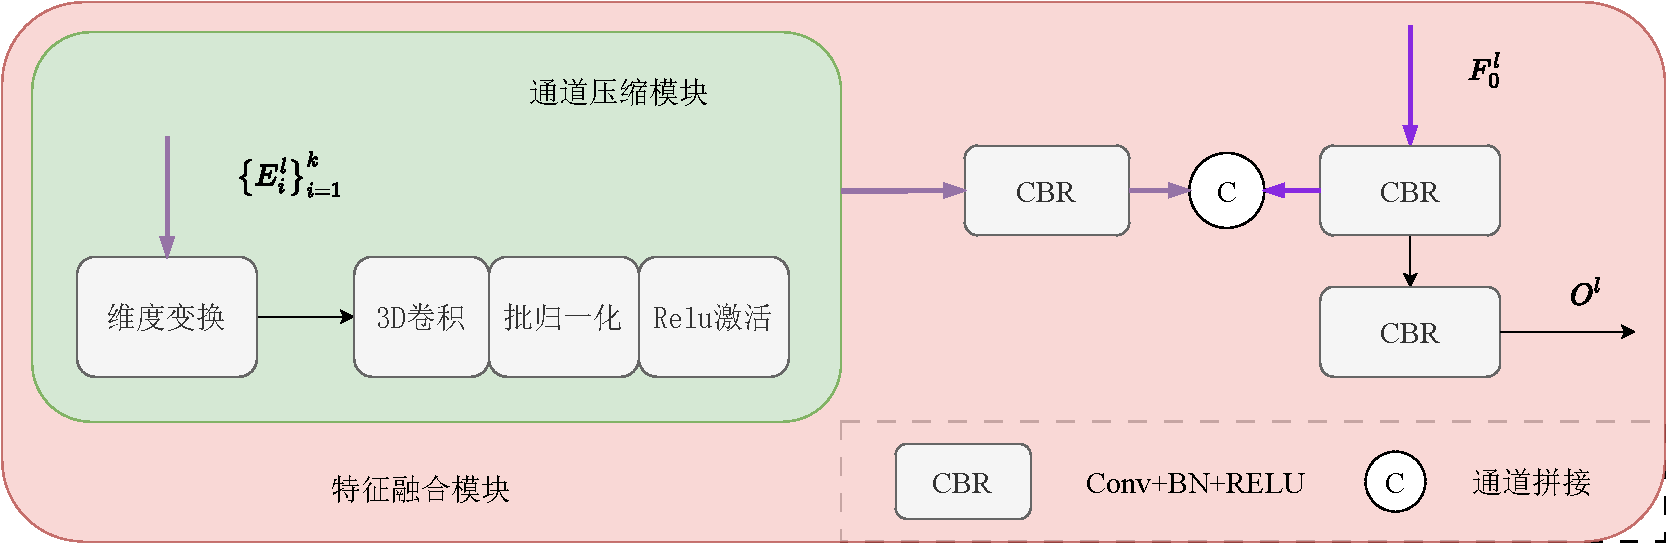
\includegraphics[width=0.95\linewidth]{figures/chapter3/ccm}
	\bicaption{特征融合模块的框架流程图}
	{Framework diagram of the feature fusion module}
%	{特征融合模块}
%	{Feature fusion module}  
	\label{cpt3_fig1:ccm}
\end{figure}




本章方法提出了一种基于 3D 卷积的通道压缩模块 (Channel Compression Module,CCM) 来解决这个问题。 
通道压缩模块引入了3D卷积,它可以本质上提取时空特征来融合所有焦点堆栈特征。
具体来说,对于形状为 $ k \times C \times h \times w $ 的每一层增强焦点堆栈特征,
将其重塑为 $ C \times  k \times  h \times w $ ,然后使用内核为 $ k \times 1 \times 1 $  的 3D 卷积来融合空间上下文特征并压缩通道。 压缩特征 $ C^{l} $ 可以表示为:
%
%
%%
%%
\begin{equation}
	C^{l} = CCM \left ( Reshape \left ( E_{1-k}^{l} \right ) \right ) ,
\end{equation}
%%
%%
%
%
其中通道压缩模块主要由3D卷积组成,包括 $3DConv+BN+RELU$。 给定与输入形状相同的焦点堆栈和全焦点特征,采用多个卷积块进行跨域融合。 因此,本章所提出的特征融合模块表述如下:
%
%
%	
%%
\begin{equation}
	%%
	O^{l}=CBR_{2}\left (Cat \left (CBR_{1} \left (F_{0}^{l} \right ),CBR_{1} \left (C^{l} \right ) \right ) \right ),
\end{equation}
%%
%%
%
%
其中 $CBR_{1}$ 和 $CBR_{2}$ 表示卷积块,包括 $Conv+BN+RELU$,前者使用 $1 \times C$ 通道输入,后者使用 $2 \times C$通道输入。
得到四层输出特征 $\left \{ O^{l} \right \}_{l=1}^{4} $ 后, 基于 FPN 的解码器\upcite{lin2017feature}生成四个显着性预测图。 
其中最后一张用作最终的显着性预测图。 
%
%
%
%
%
%\BiSubsection{损失函数}{TODO}








%%%%%%%%%%%%%%%%%%%%%%%%%%%%%%%%%%%%%%%%%%%%%%%%%%%%%%%%%%%%%%%%%%%%%%%%%%%%%%
\BiSubsection{训练过程}{Training Process}


本文所提出的网络模型使用一个混合损失函数来训练。
二元交叉熵(Binary Cross Entropy,BCE)\upcite{de2005tutorial}是二元分类和分割中使用最广泛的损失函数。 但 $\mathcal L_{bce} $ 是像素级损失,这意味着它平等对待所有像素。
在具有主导背景的图片中,前景像素的损失将会被稀释。 最近,显著性网络\upcite{qin2019basnet}中引入了交并比(Intersection over Union,IoU)损失来弥补二元交叉熵损失的不足。
$ \mathcal L_{iou} $ 的目标是优化全局结构,而不是专注于单个像素,这样就不会受到分布不平衡的影响。 增强对齐度量\upcite{fan2018enhanced}首先被提出作为一种可以同时考虑像素级和图像级误差的评估指标,
损失形式为 $ \mathcal L_{em} = 1 - E_{\xi} $。 


基于上述讨论,本章方法构建了一个混合损失:
%
%
%
%%
\begin{equation} 
	% L = L_{BCE} \left (  P,G \right )  + L_{IOU} \left ( P,G  \right ) + L_{EM} \left ( P,G  \right ) 
	\mathcal L = \mathcal L_{bce} + \mathcal L_{iou}  + \mathcal L_{em}  .
\end{equation}
%
%
%
%
\par
%
%
如图~\ref{cpt3_fig1:overview}~所示,本章所提模型有两个掩码头,它们预测辅助显着性图 $ P^{A} $ 和四个最终多尺度显着性图 $ \left \{ P_{i}^{S} \right \}_{i=1}^{4} $ 。 因此,所提出的网络的总损失 $ \mathcal L_{total} $ 可以表示为: 
%
%% 
%%
%%
\begin{equation}
	\mathcal L_{total} = \mathcal L\left ( P^{A}, G \right ) + \lambda  \sum_{i=1}^{4} \left ( \mathcal L \left (  P_{i}^{S},G \right )\right ),
	%% \mathcal L_{total} = \mathcal L\left ( T_{0}, G \right ) + \lambda  \sum_{i=0}^{3} \left ( \mathcal L \left (  P_{i}^{S},G \right )\right )
	%% \mathcal L_{total} = \mathcal L\left ( T_{0}, G \right ) + \lambda  \sum_{i=0}^{3} \left ( \mathcal L \left (  P_{i},G \right )\right )
	\label{chpt3:equ:loss_total}
\end{equation}
%%
%%
%
%
%
其中 $ G $ 表示真值图。$ \mathcal L $代表本章用来逐渐优化预测的混合损失。 $ \lambda $是用于辅助控制监督项权重的超参数。



















%%%%%%%%%%%%%%%%%%%%%%%%%%%%%%%%%%%%%%%%%%%%%%%%%%%%%%%%%%%%%%%%%%%%%%%%%%%%%%
\BiSection{实验结果与分析}{Experimental Results and Analysis}

\BiSubsection{实验设置}{Experimental Setup}



%%%%%%%%%%%%%%%%%%%%%%%%%%%%%%%%%%%%%%%%%%%%%%%%%%%%%%%%%%%%%%%%%%%%%%%%%%%%%%
(1)实验数据集


为了公平验证本章所提光场显著性目标检测算法的有效性,
采用四个公共光场基准数据集:
LFSD\upcite{li2014saliency}、
HFUT\upcite{zhang2017saliency}、
DUTLF-FS\upcite{zhang2019memory}和 
DUTLF-V2\upcite{piao2020dut}。 
HFUT 和 LFSD 相对较小,分别仅包含 255 个和 100 个样本。 
DUTLF-V2是最大的数据集,包含4204个样本,分为2957个和1247个分别用于训练和测试。 
DUTLF-FS包含1462个样本,分别分为1000个训练样本和462个测试样本。 
每个样本都包含一个全焦点图像、几个焦点切片以及相应的真值显着性图。









%%%%%%%%%%%%%%%%%%%%%%%%%%%%%%%%%%%%%%%%%%%%%%%%%%%%%%%%%%%%%%%%%%%%%%%%%%%%%%%%%%%%%
(2)实现细节



为了公平比较,本章所提方法遵循大多数以前的方法
\upcite{piao2020exploit, liu2021light}使用 DUTLF-FS 和 HFUT 的训练集来训练所提出的聚焦感知Transformer网络,
以便与使用焦点堆栈输入训练的其他光场方法进行比较。 
按照\upcite{wang2022lfbcnet,jing2021occlusion}使用 DUTLF-V2 的训练集来训练本章所提出的模型,
以便与使用多视图输入训练的其他最先进的 LFSOD 方法进行比较。 
将每个图像的大小调整为 $256 \times 256$,以便于在训练和测试中实现,
并且通过随机翻转、裁剪和旋转来增强训练数据。
使用预训练的 PVT-B2\upcite{wang2022pvt}模型初始化主干网络,
因为它具有与 ResNet50\upcite{he2016deep}相似的计算复杂性。 
本章方法共享全焦点和焦点堆栈模态之间的骨干网络权重,
以减少不必要的参数。 
整个网络使用 Adam\upcite{kingma2014adam}作为优化算法进行端到端训练,
并将初始学习率设置为 1e-4。 
小批量大小设置为 2,网络训练了 80 个循环迭代。 学习率在第 40 和 70 个迭代循环时分别乘以 0.1。 
所提出的方法是使用Pytorch工具箱\upcite{paszke2017automatic}实现的,
所有实验都在四个RTX 1080Ti GPU上进行。 



%%%%%%%%%%%%%%%%%%%%%%%%%%%%%%%%%%%%%%%%%%%%%%%%%%%%%%%%%%%%%%%%%%%%%%%%%%%%%%%%%%%%%%%%%%
(3)评价指标



本章采用了绝对平均误差、S-measure、E-measure和F-measure作为评
估模型性能的指标。




%%%%%%%%%%%%%%%%%%%%%%%%%%%%%%%%%%%%%%%%%%%%%%%%%%%%%%%%%%%%%%%%%%%%%%%%
\BiSubsection{对比实验}{Comparative Experiment}



\begin{table}[!ht]
	\bicaption{与现有显著性目标检测方法在3个光场数据集上的定量比较}
	{Quantitative comparison with existing salient object detection methods on three light field datasets}
	\centering
	\label{chpt3:table:comp_sota}
	\resizebox{\linewidth}{!}{
		\begin{tabular}{rcccccccccccc}
			\toprule[2pt]  %添加表格头部粗线
			
			% title
			%			\multirow{2}*{Type} & 
			\multicolumn{1}{c}{ \multirow{2}*{方法} } & 
			\multicolumn{4}{c}{DUTLF-FS \upcite{zhang2019memory} } &
			\multicolumn{4}{c}{HFUT \upcite{zhang2017saliency} } &
			\multicolumn{4}{c}{LFSD \upcite{li2014saliency} } \\
			
			% next line
			\cmidrule(r){2-5} \cmidrule(r){6-9} \cmidrule(r){10-13}
			
			%			 subtitle
%			& $E_{\phi}^{max}\uparrow$ & $S_{\alpha }\uparrow$ & $F_{\beta}^{max}\uparrow$ & MAE$\downarrow$ 
%			& $E_{\phi}^{max}\uparrow$ & $S_{\alpha }\uparrow$ & $F_{\beta}^{max}\uparrow$ & MAE$\downarrow$  
%			& $E_{\phi}^{max}\uparrow$ & $S_{\alpha }\uparrow$ & $F_{\beta}^{max}\uparrow$ & MAE$\downarrow$ \\
			
						& E & S & F & MAE 
						& E & S & F & MAE 
						& E & S & F & MAE \\
			
			
			% line line
			\midrule[1pt]
			
			%			\multirow{8}*{\textit{Light field}}
			
			% 开始填数据
			
			Ours	 
			&  {\textbf{.973}} & \textbf{ {.946}} 	& \textbf{ {.954}} & \textbf{ {.020}} 
			& \textbf{ {.871}} &	\textbf{ {.828}} 			&\textbf{	 {.784}} & {\textcolor{red}{.064}} 
			& \textbf{ {.919}} &	\textcolor{blue}{.860} 			&	\textbf{ {.873}} &	\textbf{ {.064}} 
			\\
			
			DLGLRG \upcite{liu2021light} 
			& {\textcolor{red}{.958}} & {\textcolor{red}{.928}} 			& {\textcolor{red}{.934}} & {\textcolor{red}{.029}} 
			&	.839 &	.766 &	.698 &	.070 
			&	{\textcolor{red}{.906}} &	\textbf{ {.866}} 			&	{\textcolor{red}{.870}} &	\textcolor{blue}{.069} 
			\\
			
			ERNet \upcite{piao2020exploit}
			& .947 & .899 & .908 & .039 
			&	.841 &	.778 &	.722 &	.082 
			&	.888 &	.834 &	.850 &	.082 
			\\
			
			PANet \upcite{piao2021panet} 
			& .939 & .908 & .903 & .038 
			& .845 & .795 & .738 & .074 
			& .892 & .849 & .849 & .076
			\\
			
			LFNet	 \upcite{zhang2020lfnet} 
			& .929 & .878 & .890 & .053
			&	.846 &	.782 &	.718 &	.073 
			&	.885 &	.820 &	.824 &	.092 \\
			
			MAC	 \upcite{zhang2020light} 
			& .863	& .804	& .792	& .102	
			&   .797 & .731 & .667 & .107 
			& .832 & .782 & .776 & .127 \\
			
			MoLF	 \upcite{zhang2019memory} 
			& .938 & .887 & .902 & .051 
			&	.852 &	.789 &	.729 &	.075 
			&	.888 &	.830 &	.834 &	.089 \\
			
			DLSD	\upcite{piao2019deep}
			& .891	& .841	& .801	& .076	
			&   .783 & .741 & .615 & .098 
			& .806 & .737 & .715 & .147 \\
			
			\midrule[1pt] % end lfsod
			
			% start rgb-d
			%			\multirow{6}*{\textit{RGB-D}}
			
			DCF \upcite{ji2021calibrated} 
			& \textcolor{blue}{.954} & \textcolor{blue}{.921} & \textcolor{blue}{.927} & \textcolor{blue}{.031} 
			& \textcolor{blue}{.856} & {\textcolor{red}{.812}} & {\textcolor{red}{.768}} & \textcolor{blue}{.065} 
			& .881 & .809 & .821 & .096 \\
			
			CIR-Net \upcite{cong2022cir}
			& .950 & .916 & .921 & .038 
			& {\textcolor{red}{.862}} & .800  			& .742 & \textbf{ {.062}} 
			& .874 & .820 & .816 & .098 \\ 
			
			VST-$rgbd$  \upcite{liu2021visual} 
			& .952 & .920 & .921 & .036 
			& .843 & .807 & .754 & .086 
			& .851 & .792 & .786 & .110 
			\\
			
			%			& -  & 2022  & \\
			%			& -  & 2022  & \\
			
			BBS-Net     \upcite{fan2020bbs} 
			& .900 & .865 & .852 & .066 
			& .801 & .751 & .676 & .073 
			& \textcolor{blue}{.901} & {\textcolor{red}{.864}} & .858 & .072 \\ 
			
			SSF     \upcite{zhang2020select} 
			& .922 & .879 & .887 & .050 
			& .816 & .725 & .647 & .090 
			& \textcolor{blue}{.901} & .859 & \textcolor{blue}{.868} & {\textcolor{red}{.067}} \\ 
			
			S2MA    \upcite{liu2020learning} 
			& .839 & .787 & .754 & 	.102 
			& .777 & .729 & .650 & .112 
			& .873 & .837 &	.835 & .094 \\
			
			
			\midrule[1pt] 
			
			%			\multirow{7}*{\textit{RGB}}
			
			VST-$rgb$ \upcite{liu2021visual} 
			& .939 & .910 & .911 & .047
			& .831 & \textcolor{blue}{.808} & \textcolor{blue}{.763} & .093 
			& .865 & .797 & .817 & .123 
			\\ 
			
			PFSNet \upcite{ma2021pyramidal}
			& .912 & .883 & .879 & .057 
			& .835 & .800 & .752 & .088 
			& .805 & .749 & .727 & .145 
			\\ 
			
			
			ITSD \upcite{zhou2020interactive} 
			& .930 & .899 & .899 & .052 
			& .839 & .805 & .759 & .089 
			& .879 & .847 & .840 & .088 
			\\ 
			
			
			
			LDF \upcite{wei2020label} 
			& .898 & .873 & .861 & .061 
			& .804 & .780 & .708 & .093 
			& .843 & .821 & .803 & .096 
			\\ 
			
			
			MINet \upcite{pang2020multi} 
			& .916 & .890 & .882 & .050 
			& .816 & .792 & .720 & .086 
			& .861 & .834 & .828 & .091 
			\\ 
			
			F$^{3}$Net  \upcite{wei2020f3net}
			& .900 & .888 & .882 & .057 
			& .815 & .777 & .718 & .095 
			& .824 & .806 & .797 & .106 
			\\ 
			
			
			EGNet   \upcite{zhao2019egnet}
			& .914 & .886 & .870 & .053 
			& .794 & .772 & .672 & .094 
			& .776 & .784 & .762 & .118 
			\\ 
			
			CPD  \upcite{wu2019cascaded}
			& .867 & .911 & .866 & .058 
			& .772 & .82  & .701 & .086 
			& .759 & .82  & .759 & .126 \\
			
			PoolNet \upcite{liu2019simple}
			& .889 & .919 & .868 & .051 
			& .776 & .802 & .683 & .092 
			& .789 & .8   & .769 & .118 \\
			
			PiCANet \upcite{liu2018picanet}
			& .829 & .892 & .821 & .083 
			& .726 & .781 & .618 & .115 
			& .729 & .78  & .671 & .158 \\
			
			PAGRN \upcite{wang2018detect}
			& .822 & .878 & .828 & .084 
			& .717 & .773 & .635 & .114 
			& .727 & .805 & .725 & .147 \\
			
			C2S   \upcite{li2018contour}
			& .844 & .874 & .791 & .084 
			& .763 & .786 & .65  & .111 
			& .806 & .82  & .749 & .113 \\
			
			R3Net  \upcite{deng2018r3net}
			& .833 & .819 & .783 & .113 
			& .727 & .728 & .625 & .151 
			& .789 & .838 & .781 & .128 \\
			
			Amulet \upcite{zhang2017amulet}
			& .847 & .882 & .805 & .030 
			& .767 & .76  & .636 & .110  
			& .773 & .821 & .757 & .135 \\
			
			
			\bottomrule[2pt] % end
		\end{tabular}
	}
	%	\vspace{3cm}
\end{table}



%---------------------------------------------------------------------> 消融实验: 多视角方法对比
%
\begin{table}[t]
	\bicaption{与多视角光场显著性目标检测方法比较的定量结果}
	{Quantitative results of comparison with multi-view light field salient object detection methods}
	\centering
	\label{table:comp_multi_view}
	%	\resizebox{\linewidth}{!}{
		\begin{tabular}{crcccc}
			\toprule[2pt]  %添加表格头部粗线
			
			% title
			\multirow{2}*{输入类型} & \multicolumn{1}{c}{\multirow{2}*{方法}} & \multicolumn{4}{c}{DUTLF-V2 \upcite{piao2020dut}} \\
			
			% next line
			\cmidrule(r){3-6} 
			
			% subtitle
			& & $E_{\phi}^{max}\uparrow$ & $S_{\alpha }\uparrow$ & $F_{\beta}^{max}\uparrow$ & MAE$\downarrow$ \\
			
			\midrule[1pt]  % E S F MAE
			
			焦点堆栈       & \multicolumn{1}{c}{ Ours$^{\ast} $ } &
			\textbf{ 0.960 } & \textbf{ 0.923 }  & \textbf{ 0.917 }  & \textbf{ 0.026 }  \\ 
			%								 &  0.9598 & 0.9227 & 0.9173 & 0.0256 \\
			% multiview
			
			\midrule[1pt]
			
			\multirow{3}*{多视角图}
			& OBGNet \upcite{jing2021occlusion}      &  0.940  & 0.896  & 0.885  & 0.037  \\
			& LFBCNet \upcite{wang2022lfbcnet}    &  0.940  & 0.890  & 0.870  & -      \\
			& ESCNet \upcite{zhang2022exploring}      &  0.931  & 0.882  & 0.852  & 0.041  \\
			
			
			\bottomrule[2pt]
		\end{tabular}
		%}
\end{table}






%%%%%%%%%%%%%%%%%%%%%%%%%%%%%%%%%%%%%%%%%%%%%%%%%%%%%%%%%%%%%%%%%%%%%%%%%%%%%%%%%%%%%%%%%%%%
(1)定量比较

为了进行全面比较,本章方法将与 26 个最先进的光场显著性目标检测模型进行比较,
包括6个光场显著性分割方法:
DLGLRG \upcite{liu2021light}, RENet \upcite{piao2020exploit}, LFNet \upcite{zhang2020lfnet},
MAC \upcite{zhang2020light}, MoLF \upcite{zhang2019memory}, and DLSD \upcite{piao2019deep};
%
%
%
%
6个RGB-D显著性分割方法:
DCF \upcite{ji2021calibrated}, CIR-Net \upcite{cong2022cir}, VST-$rgbd$  \upcite{liu2021visual},
BBS-Net     \upcite{fan2020bbs}, SSF     \upcite{zhang2020select} and S2MA    \upcite{liu2020learning};
%
%
%
%
%
和14个2D显著性检测方法:
VST-$rgb$ \upcite{liu2021visual},
PFSNet \upcite{ma2021pyramidal},
ITSD \upcite{zhou2020interactive},
LDF \upcite{wei2020label},
MINet \upcite{pang2020multi},
F$^{3}$Net  \upcite{wei2020f3net}, 
EGNet   \upcite{zhao2019egnet},
CPD  \upcite{wu2019cascaded},
PoolNet \upcite{liu2019simple},
PiCANet \upcite{liu2018picanet},
PAGRN \upcite{wang2018detect},
C2S   \upcite{li2018contour},
R3Net  \upcite{deng2018r3net}
和
Amulet \upcite{zhang2017amulet}。






为了保证公平比较,使用上述方法所提供的显着性预测图或预训练的权重来生成比较数据,
并利用\upcite{liu2021visual}提供的相同评估代码。
如表~\ref{chpt3:table:comp_sota}~所示,
很明显,所提出的方法在 DUTLF-FS 和 HFUT 数据集上实现了比当前最先进的方法更优越的性能。 同时,所提出的方法可以在除了 $ S_{\alpha} $ 的另外三个指标上超越其他方法。 值得一提的是,与使用大量数据集训练的 RGBD 和 RGB 的显著性检测方法相比,本章方法在小三倍的训练集(1100 vs. 2985 vs. 10553)下取得了显着的优势。 
这表明本章所提方法可以有效地探索光场数据中传达的信息。 



为了检验本章方法与其他使用不同光场数据输入的网络模型的性能差异,
在 DUTLF-V2 上重新训练本章方法,
并与其他三种使用多视图图像作为输入的光场显著性目标分割方法进行比较,
包括 OBGNet\upcite{jing2021occlusion}、
LFBCNet\upcite{wang2022lfbcnet}和
ESCNet\upcite{zhang2022exploring}。 
如表~\ref{table:comp_multi_view}~所示,
本章方法可以在 DUTLF-V2 的所有四个指标上大幅实现最佳性能。 
这证明了本章所提网络对于使用焦点堆栈作为输入的有效性以及信息提取方式的高效性。 






%%%%%%%%%%%%%%%%%%%%%%%%%%%%%%%%%%%%%%%%%%%%%%%%%%%%%%%%%%%%%%%%%%%%%%%%%%%%%%%%%%%%%%%%%%%
(2)定性比较:


为了更直观地观察,
图~\ref{figure:figure_comparison_1}~和
~\ref{figure:figure_comparison_2}~
中可视化了所提出的方法和其他排名靠前的方法生成的一些代表性结果。
其中图~\ref{figure:figure_comparison_1}~中,
可视化对比了本章方法和5个其他光场显著性检测方法的显著性预测结果。
在图~\ref{figure:figure_comparison_2}~中,
可视化了本章方法、2个RGB-D显著性检测方法和
2个RGB显著性检测方法的显著性预测结果。
可以看出,本章所提出的方法的结果与真值图更加一致。 
当面对这些具有挑战性的场景时,
包括多个对象(第 4、5 行)和复杂场景(第 6、7 行),
大多数 RGB 和 RGB-D 显著性检测方法无法准确检测显着对象。
相比之下,本章所提出的方法可以成功生成准确且稳健的显着图。
与这些基于卷积神经网络的光场显著性目标检测方法相比,
所提出的方法获得了更一致的预测结果和更精细的细节。




\begin{figure}[b]
	\centering
	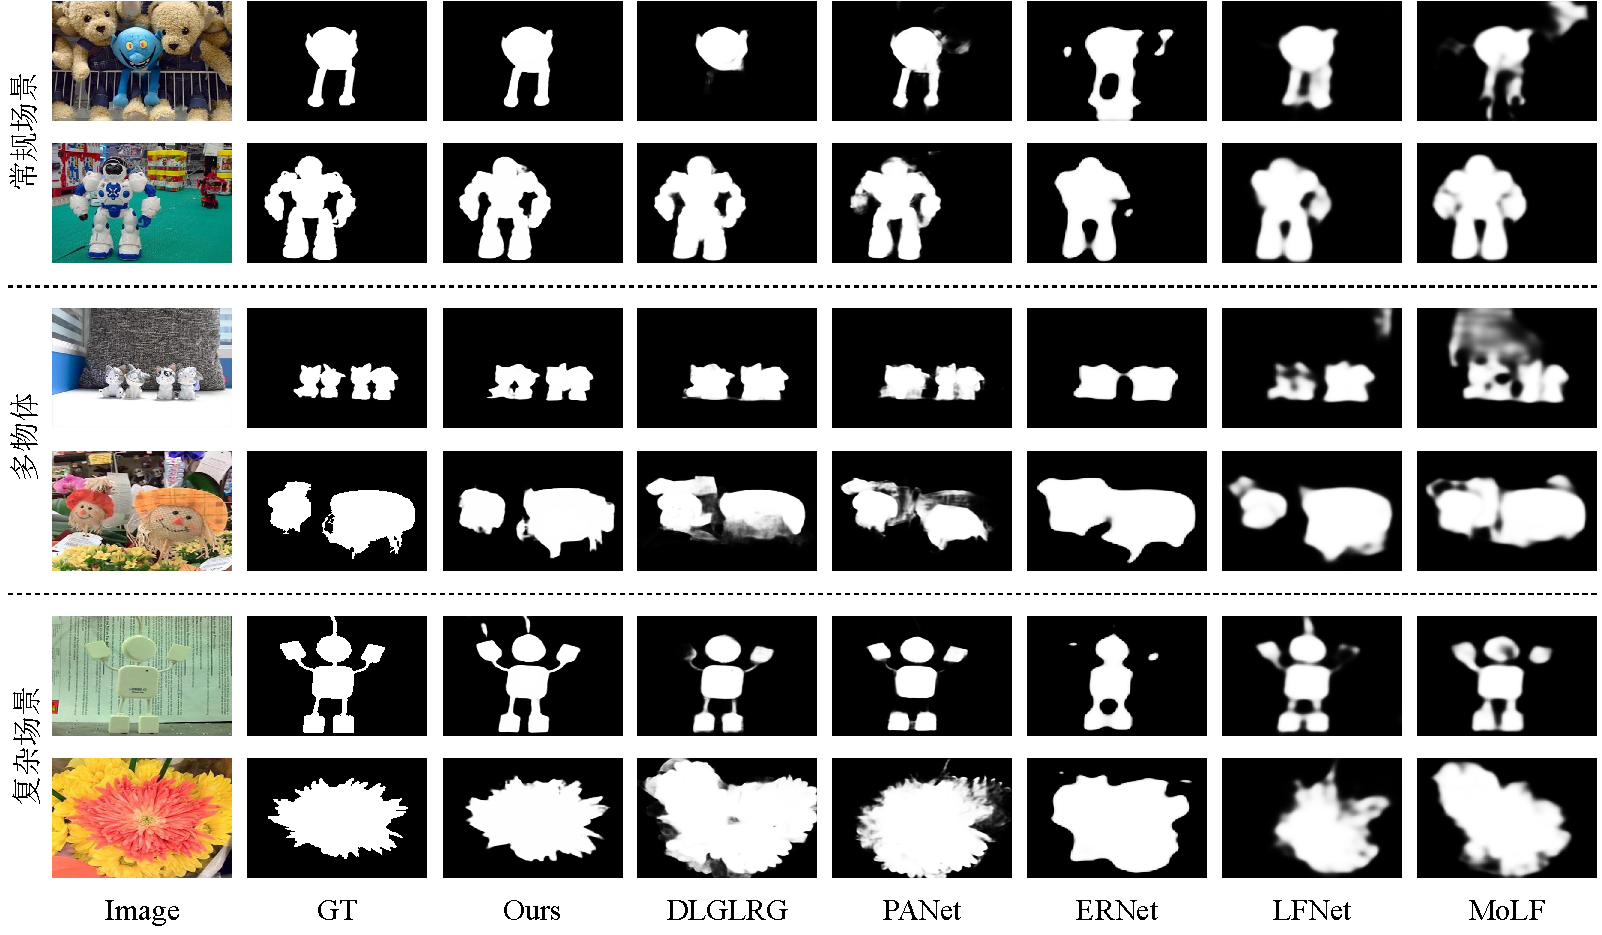
\includegraphics[width=\linewidth]{figures/chapter3/compare_1}
	\bicaption{在一些具有挑战性的场景中与最先进方法的可视化比较}
	{Visual comparisons with state-of-the-art methods in challenging scenes}
	\label{figure:figure_comparison_1}
\end{figure}


\begin{figure}[!ht]
	\centering
	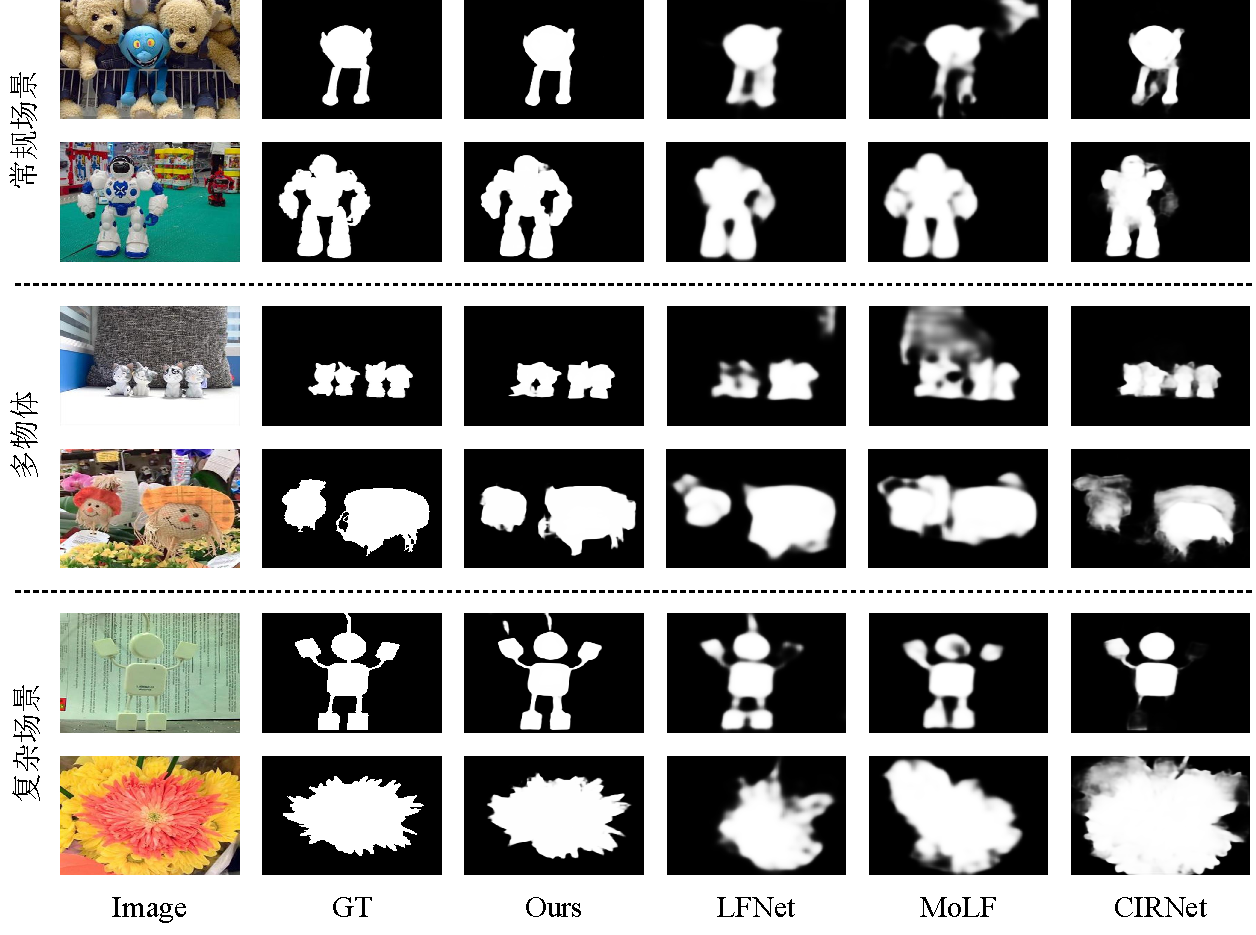
\includegraphics[width=\linewidth]{figures/chapter3/compare_2}
	\bicaption{挑战性场景下与其它显著性目标检测方法的可视化比较}
	{Visual comparisons with other salient object detection methods in challenging scenarios}
	%	{在一些具有挑战性的场景中与最先进的方法的可视化比较}
	%	{Visual comparisons with state-of-the-art methods in challenging scenes}
	\label{figure:figure_comparison_2}
\end{figure}





%%%%%%%%%%%%%%%%%%%%%%%%%%%%%%%%%%%%%%%%%%%%%%%%%%%%%%%%%%%%%%%%%%%%%%%%%%%%%%%%%%%%%%%%%%%%%
\BiSubsection{消融实验}{Ablation Experiment}


%%%%%%%%%%%%%%%%%%%%%%%%%%%%%%%%%%%%%%%%%%%%%%%%%%%%%%%%%%%%%%%%%%%%%%%%%%%%%%%%%%%%%%%%%%%%%
(1)
不同模型组件的有效性
%\textbf{不同模型组件的有效性。}



本节在表~\ref{table:abl_total}~中验证不同模型组件的有效性。
首先构建一个基线模型。 
具体来说,它使用共享权重编码器来提取全聚焦图和焦点堆栈特征,
然后在通道维度进行拼接,送入使用二维卷积网络构建的融合模块进行进一步的特征提取,
最后将融合后的特征送入显著性目标检测头并预测最终的显著性图。 







%%%%%%%%%%%%%%%%%%%%%%%%%%%%%%%%%%%%%%%%%%%%%%%%%%%
%%
%% Split paragraphs
%%
%%%%%%%%%%%%%%%%%%%%%%%%%%%%%%%%%%%%%%%%%%%%%%%%%%%



本章设置了多个实验来验证所提模块的有效性,
具体来说,
逐渐在基线网络中添加令牌通信模块,聚焦感知增强策略和特征融合模块
到本章所提的聚焦感知网络中,在表~\ref{table:abl_total}~中分别以标号2,~4,~5表示。
如表~\ref{table:abl_total}~所示,这三个模型可以逐渐提高光场显著性目标检测性能,
最终大幅优于基线模型。 


\begin{table}[t]
	\bicaption{本章方法在DUTLF-FS数据集上的消融实验结果}
	{Ablation experimental results of the proposed method on the DUTLF-FS dataset}
	%	{在 DUTLF-FS 数据集上每个组件的消融分析}
	%	{Ablation analyses of each component on the DUTLF-FS dataset}
	\centering
	\label{table:abl_total}
	\label{chpt3:table:abl_total}
	%	\resizebox{0.82\linewidth}{!}{
		\begin{tabular}{cllcccc}
			\toprule[2pt]  %添加表格头部粗线
			%%  \multicolumn{1}{c}{ \multirow{2}*{Methods} }
			
			\multicolumn{1}{c}{ \multirow{2}*{实验编号}} 
			& \multicolumn{2}{c}{ \multirow{2}*{设置}}	
			& \multicolumn{4}{c}{DUTLF-FS} \\
			
			\cmidrule(r){4-7} 
			
			& & & $E_{\phi}^{max}\uparrow$ & $S_{\alpha }\uparrow $ & $F_{\beta}^{max}\uparrow$ & MAE$\downarrow$ \\
			
			
			\midrule
			
			%			% 开始填写数据
			1 & \multicolumn{2}{l}{ Baseline }     & 0.947 & 0.894 & 0.901 & 0.048 \\ 
			
			%		 			\multicolumn{2}{l}{+Token} 	 & 0.959 & 0.918 & 0.926 & 0.037 \\ 
			
			\midrule
			
			2 & \multicolumn{1}{l}{ \multirow{2}*{+令牌通信模块}}	
			
			& \multicolumn{1}{c}{+令牌交互操作}  & 0.961 & 0.923 & 0.932 & 0.034 \\ 
			3 & & \multicolumn{1}{c}{++令牌移位操作} & 0.968 & 0.933 & 0.944 & 0.027 \\
			
			\midrule
			
			4 & \multicolumn{2}{l}{++~~~聚焦感知增强} 		
			& \textbf{0.972} & 0.941 & 0.952 & 0.022 \\
			
			5 & \multicolumn{2}{l}{+++特征融合模块} 		
			& \textbf{0.972} & \textbf{0.942} & \textbf{0.953} & \textbf{0.021} \\ 
			
			
			\bottomrule[2pt]
		\end{tabular}
		% }
\end{table}


\begin{figure}[b] 
	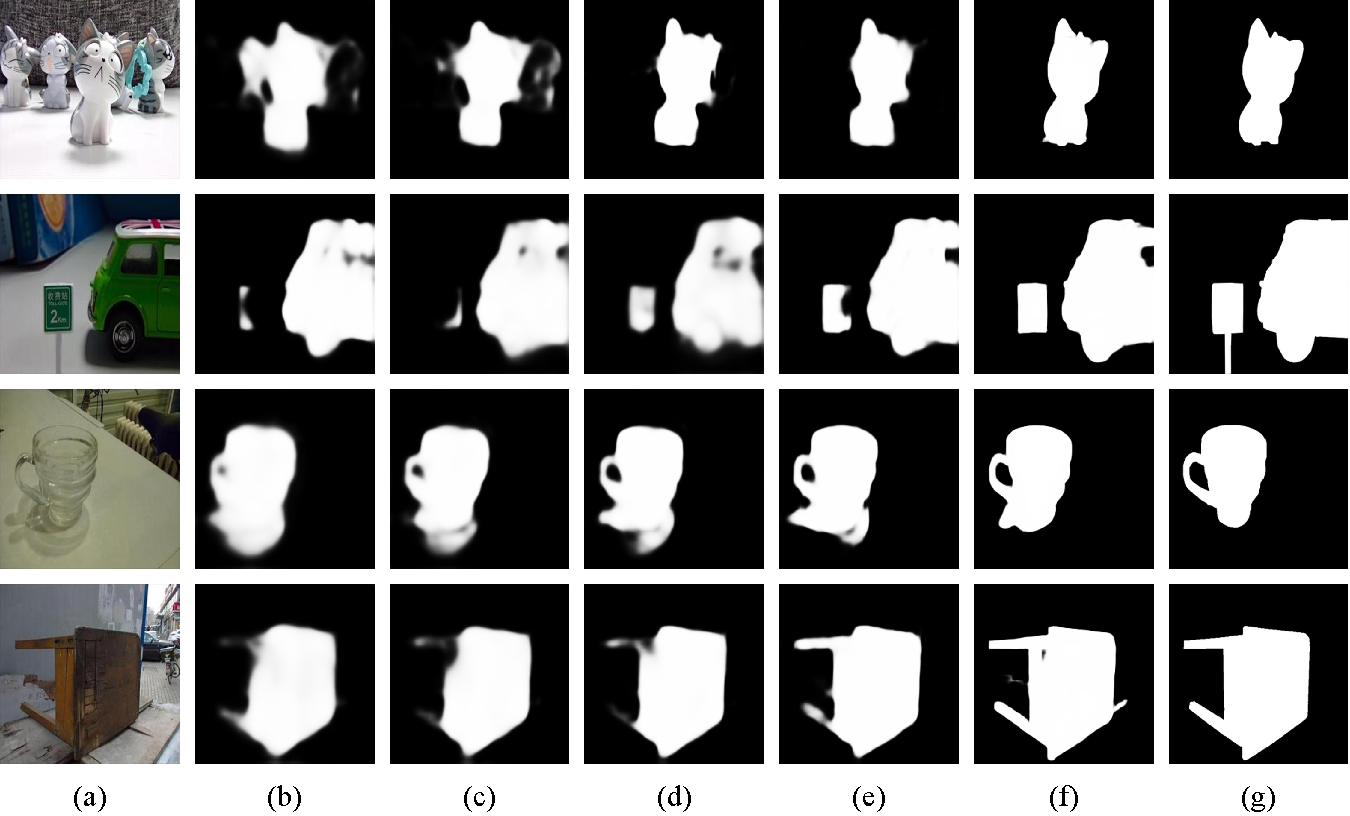
\includegraphics[width=0.99\linewidth]{figures/chapter3/self-comparsion-Use} 
	\centering
	\bicaption{消融实验的可视化结果}
	{Visualized results of ablation experiments}
	%	{消融研究的可视化比较}
	%	{Visual comparisons of ablation studies}
	\label{figure:self_comp}
\end{figure}



\begin{table}[!ht]
	\bicaption{焦点相关令牌数量的影响, $M$表示焦点相关令牌的数量}
	{Impact of focal-related token numbers. $M$ indicates the number of focal-related tokens}
	\centering
	\label{table:abl_token_number}
		\resizebox{0.40\linewidth}{!}{
		\begin{tabular}{ccccc}
			\toprule[2pt]  %添加表格头部粗线
			
			% title
			\multirow{2}*{$M$} & \multicolumn{4}{c}{DUTLF-FS} \\ % & \multicolumn{3}{c}{HFUT} \\
			
			% next line
			\cmidrule(r){2-5} % \cmidrule(r){5-7} % \cmidrule(r){7-8} 
			
			% subtitle
			& $E_{\phi}^{max}\uparrow$ & $S_{\alpha }\uparrow $ & $F_{\beta}^{max}\uparrow$ & MAE$\downarrow$\\
			% & $S_{\alpha }\uparrow $ & $F_{\beta}^{max}\uparrow$ & MAE$\downarrow$ \\
			
			\midrule
			
			% 开始填写数据
			%% 8 & 0.969 & 0.934 & 0.944 & 0.026 \\ 
			
			8 &  0.967 & 0.936 & 0.946 & 0.025 \\ 
			16 & 0.970 & 0.937 & 0.948 & 0.024 \\
			32 & \textbf{0.972} & \textbf{0.941} & \textbf{0.952} & \textbf{0.022} \\ 
			
			\bottomrule[2pt]
		\end{tabular}
			}
	
\end{table}


\begin{table}[!ht]
	\bicaption{聚焦感知增强策略中使用不同$K$数的比较}
	{Comparison of using different $K$ numbers in focal perception enhancement strategy}
	\centering
	\label{table:abl_fp}
		\resizebox{0.42\linewidth}{!}{
		\begin{tabular}{ccccc}
			\toprule[2pt]  %添加表格头部粗线
			
			% title
			\multirow{2}*{K} & \multicolumn{4}{c}{DUTLF-FS} \\ % & \multicolumn{3}{c}{HFUT} \\
			
			% next line
			\cmidrule(r){2-5} % \cmidrule(r){5-7} % \cmidrule(r){7-8} 
			
			% subtitle
			& $E_{\phi}^{max}\uparrow$ & $S_{\alpha }\uparrow $ & $F_{\beta}^{max}\uparrow$ & MAE$\downarrow$\\
			% & $S_{\alpha }\uparrow $ & $F_{\beta}^{max}\uparrow$ & MAE$\downarrow$ \\
			
			\midrule
			
			% 开始填写数据
			1 & 0.969 & 0.934 & 0.944 & 0.026 \\ 
			3 & 0.969 & 0.937 & 0.947 & 0.024 \\ 
			5 & \textbf{0.972} & \textbf{0.941} & \textbf{0.952} & \textbf{0.022} \\ 
			7 & 0.971 & 0.940 & 0.951 & \textbf{0.022} \\ 
			9 & 0.971 & 0.938 & 0.951 & 0.023 \\ 
			
			\bottomrule[2pt]
		\end{tabular}
			}
\end{table}


\begin{table}[!ht]
	\bicaption{聚焦感知增强策略中不同方法的消融结果}
	{Ablation results of different methods for focal perception enhancement module}
	%	{FPEM中不同方法的消融结果}
	%	{Ablation results of different methods for FPEM}
	
	\centering
	\label{table:abl_methods}
		\resizebox{0.60\linewidth}{!}{
		\begin{tabular}{ccccc}
			\toprule[2pt]  %添加表格头部粗线
			
			% title
			\multirow{2}*{实验设置} & \multicolumn{4}{c}{DUTLF-FS} \\  % & \multicolumn{3}{c}{HFUT} \\
			
			% next line
			\cmidrule(r){2-5} % \cmidrule(r){5-7} % \cmidrule(r){7-8} 
			
			% subtitle
			& $E_{\phi}^{max}\uparrow$ & $S_{\alpha }\uparrow $ & $F_{\beta}^{max}\uparrow$ & MAE$\downarrow$ \\
			% & $S_{\alpha }\uparrow $ & $F_{\beta}^{max}\uparrow$ & MAE$\downarrow$ \\
			
			\midrule
			
			% 开始填写数据
			随机增强      & 0.962 & 0.924 & 0.932 & 0.033 \\ 
			卷积增强        & 0.967 & 0.931 & 0.942 & 0.027 \\ 
			结构相似度增强        & \textbf{0.972} & \textbf{0.941} & \textbf{0.952} & \textbf{0.022} \\ 
			%% Log(SSIM)   & \textbf{0.972} & 0.940 & 0.950 & 0.023 \\ 
			
			\bottomrule[2pt]
		\end{tabular}
		}
\end{table}




此外,为了证明本章所提出的令牌通信模块中的令牌交互操作和令牌移位操作的有效性,
在表~\ref{table:abl_total}~中添加标号为2,3的网络,
分别表示只在基线模型上添加令牌交互操作,以及基于模型2,再添加令牌移位操作的网络。
从表中数据可以看出,与标号1的基线模型相比。
模型2和模型3在 DUTLF-FS 数据集上分别使 MAE 指标降低 29.2\% 和 43.8\%。 




%%%%%%%%%%%%%%%%%%%%%%%%%%%%%%%%%%%%%%%%%%%%%%%%%%%%%%%%%%%%%%%%%%%%%%%%%%%%%%%%%%
本节还在图~\ref{figure:self_comp}~中提供了每个消融研究相应的可视化结果,
其中(a)表示全聚焦图像,
(b)-(f) 分别代表基线模型、以及在基线模型基础上逐步添加
令牌交互操作,令牌移位操作、聚焦感知增强策略和特征融合模块的显著性目标预测图,
对应消融实验表~\ref{chpt3:table:abl_total}~中编号从1-5的不同设置的方法。
可以发现,预测的二进制掩码表示与真值图逐渐变得更加一致。 
显着对象的完整内容和精确的显着图边界,
证明本章所提出的聚焦感知Transformer模型可以有效过滤掉背景干扰并更多地关注显着对象。 






 

%\textbf{焦点相关标记的数量。} 


%%%%%%%%%%%%%%%%%%%%%%%%%%%%%%%%%%%%%%%%%%%%%%%%%%%%%%%%%%%%%%%%%%%%%%%%%%%%%%%%%%%%%%%%%%%%%
(2)
焦点相关标记的数量



在表~\ref{table:abl_token_number}~中,采用不同的与焦点相关标记的数量来设计实验,
标记数量从 8 个增加到 32 个来测试本章方法。
与使用较少的焦点相关标记 ($M$ = 8, 16) 相比,使用更多的焦点相关标记 ($M$ = 32) 可以获得更好的结果 。 
除非另有说明,本章的实验均使用 32 个与焦点相关的标记。 




%%%%%%%%%%%%%%%%%%%%%%%%%%%%%%%%%%%%%%%%%%%%%%%%%%%%%%%%%%%%%%%%%%%%%%%%%%%%%%%%%%



%%%%%%%%%%%%%%%%%%%%%%%%%%%%%%%%%%%%%%%%%%%%%%%%%%%%%%%%%%%%%%%%%%%%%%%%%%%%%%%%%%%%%%%%%%%%%
(3)
聚焦感知增强策略中的 $K$ 值


本章设置了多个比较实验来选择最佳 $k$ 数,具体数据见表~\ref{table:abl_fp}。
将 $K$ 从 1 增加到 5 时,性能逐渐提高。 
当 $K > 5$ 时,观察到模型性能饱和并变得次优。 
分析认为较大的 $K$ 值会引入更多不显着的背景效应。 
考虑到性能和计算成本之间的权衡,本章方法选择 $K = 5$ 作为最终配置。


%%%%%%%%%%%%%%%%%%%%%%%%%%%%%%%%%%%%%%%%%%%%%%%%%%%%%%%%%%%%%%%%%%%%%%%%%%%%%%%%%%%%%%%%%%%%%
(4)
聚焦感知增强方法设置



为了验证不同聚焦感知增强设置的有效性,
本章方法在随机、卷积和基于 SSIM 的选择方法之间进行了比较实验。 
所有实验将 $K$ 数设置为 5。
表~\ref{table:abl_methods}~中所示,
本章方法在使用基于卷积方式进行感知增强时已经达到了与其他光场显著性目标检测方法相当的性能,
证明了本章所提出方法的优越性。



%%%%%%%%%%%%%%%%%%%%%%%%%%%%%%%%%%%%%%%%%%%%%%%%%%%%%%%%%%%%%%%%%%%%%%%%%%%%%%%%%%%%%%%%%%%%%
\BiSection{本章小结}{The Chapter’s Conclusion}

在本章中,提出了一种用于精确光场显着物体检测的聚焦感知Transformer(FPT)。 
通过引入与焦点相关的令牌来收集图像特定的特征,并提出令牌通信模块(TCM)来传播信息并促进空间上下文建模。 
为了增强焦点堆栈的空间特征表示,本章提出了一种聚焦感知增强(FPE)策略来帮助抑制噪声背景信息。 
实验结果表明,本章所提出的方法可以在大多数光场显著性分割数据集上实现最先进的性能。